Drei homogene Quader stehen auf einer schiefen Ebene mit dem Neigungswinkel $\alpha = \alO$. Die Ebene ist so rau, dass keiner rutscht. Ihre Abmessungen (Breite $b$ entlang der Ebene, Höhe $h$ senkrecht zur Ebene):
\begin{center}
\begin{tabular}{lccc}
 Quader & A & B & C \\ \hline
 Breite $b$ & \wAO & \wBO & \wCO \\
 Höhe $h$ & \hAO & \hBO & \hCO
\end{tabular}
\end{center}
\begin{center}
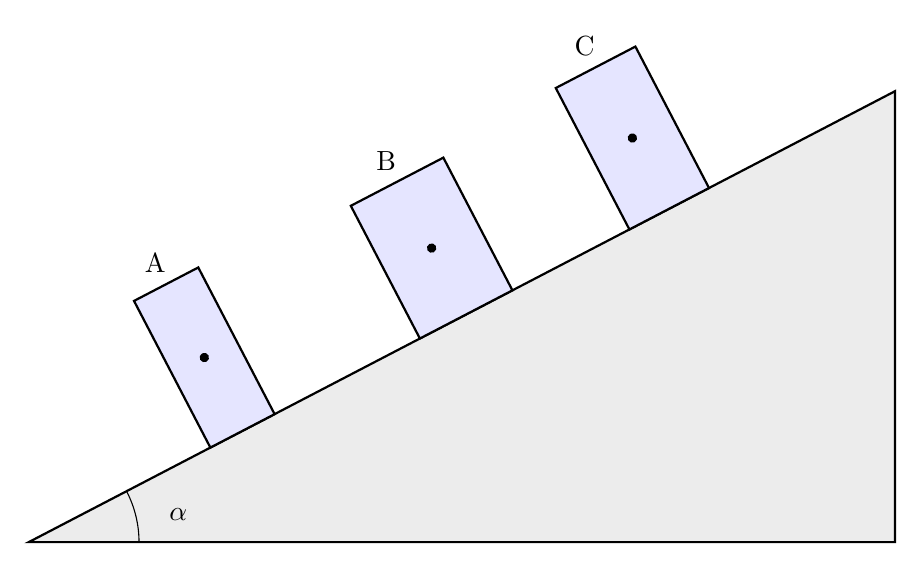
\begin{tikzpicture}[scale=1]
 \draw[thick, fill=gray!15] (0,0) -- (11,0) -- (11,5.726) -- cycle;
 \draw (1.4,0) arc (0:27.5:1.4); \node at (1.9,0.35) {$\alpha$};
 \foreach \s/\w/\h/\n in {2.6/0.92/2.10/A, 5.6/1.325/1.90/B, 8.6/1.14/2.025/C} {
  \begin{scope}[rotate=27.5, shift={(\s,0)}]
   \draw[thick, fill=blue!10] (0,0) rectangle (\w,\h);
   \fill (\w/2,\h/2) circle (0.06);
   \node at (\w/2,\h+0.3) {\n};
  \end{scope}
 }
\end{tikzpicture}
\end{center}

\begin{abcliste}
\abc
Um welche Kante würde ein Quader kippen? \DuSie{Zeige}{Zeigen Sie}: Er kippt, wenn
\[
 \tan\alpha > \frac{b/2}{h_\mathrm{S}}
\]
ist, wobei $h_\mathrm{S}$ die Höhe des Schwerpunkts über der Grundfläche ist.

\abc
Welche der drei Quader kippen um?

\abc
Bei welchem Neigungswinkel würde jeder Quader zu kippen beginnen?
\end{abcliste}
